\section{Analisi dei rischi} \label{section:analisi_dei_rischi}
Questa sezione presenta un'analisi approfondita dei possibili rischi in cui si potrebbe incorrere durante l'avanzamento del progetto.\\
Per il corretto trattamento dei rischi viene attuata la seguente procedura:
\begin{itemize}
  \item \textbf{Identificazione:} Individuare i potenziali rischi e comprendere com'è possibile rilevarli;
  \item \textbf{Analisi:} Valutare la probabilità che si verifichi e le conseguenze che tale rischio comporterebbe;
  \item \textbf{Piano di contingenza:} Fornisce la modalità di mitigazione qualora il rischio dovesse verificarsi.
\end{itemize}
Per informazioni relative alla codifica dei rischi, fare riferimento alle \docNameVersionNdP{}.\\
È stato deciso di suddividere i rischi individuati, con relativa occorrenza (Alta (A), Media (M), Bassa (B)), nelle seguenti categorie:

%%%%%%%%%%%%%%%%%%%%%%%%%%%%%%%%%%%%%%%%%%%%%%%%%%%%%%%%%%%%%%%%%%%%%%%%%%%%%%%%%%%%%%%%%%%%%%%%%%%%
\subsection{Rischi tecnologici} \label{subsection:rischi_tecnologici}
\begin{table}[H]
  \centering
  \renewcommand{\arraystretch}{1.8}
  \rowcolors{2}{green!100!black!40}{green!100!black!30}
  \begin{tabular}{p{5.5cm}|p{5cm}|p{5cm}|c}
    \rowcolor[HTML]{125E28} 
    \multicolumn{1}{c}{\color[HTML]{FFFFFF}\textbf{Codice}}
    & \multicolumn{1}{c}{\color[HTML]{FFFFFF}\textbf{Descrizione}}
    & \multicolumn{1}{c}{\color[HTML]{FFFFFF}\textbf{Identificazione}}
    & \color[HTML]{FFFFFF}\textbf{Occ.}\\
    \hline
    \textbf{RT1} - Inesperienza tecnologica & È legato alla difficoltà di utilizzo di tecnologie sconosciute ai componenti del gruppo. & Sarà compito di tutti i membri del gruppo rilevare la necessità di utilizzare tecnologie sconosciute ai più, in particolare sarà il \roleProjectManagerLow{} a dover prestare maggior attenzione. & A \\
    \textbf{RT2} - Problemi hardware o software & Si presenta se per qualsiasi motivo uno strumento di lavoro di un componente del gruppo non permette lo svolgimento di qualche attività o lo permette solo in parte. &  Sarà compito di chi incorrerà in questo rischio farlo presente agli altri membri del gruppo. & M \\
  \end{tabular}
  \caption{Rischi tecnologici}
\end{table}

%%%%%%%%%%%%%%%%%%%%%%%%%%%%%%%%%%%%%%%%%%%%%%%%%%%%%%%%%%%%%%%%%%%%%%%%%%%%%%%%%%%%%%%%%%%%%%%%%%%%%
\subsection{Rischi interni} \label{subsection:rischi_interni}
\begin{table}[H]
  \centering
  \renewcommand{\arraystretch}{1.8}
  \rowcolors{2}{green!100!black!40}{green!100!black!30}
  \begin{tabular}{p{5.5cm}|p{5cm}|p{5cm}|c}
    \rowcolor[HTML]{125E28} 
    \multicolumn{1}{c}{\color[HTML]{FFFFFF}\textbf{Codice}}
    & \multicolumn{1}{c}{\color[HTML]{FFFFFF}\textbf{Descrizione}}
    & \multicolumn{1}{c}{\color[HTML]{FFFFFF}\textbf{Identificazione}}
    & \color[HTML]{FFFFFF}\textbf{Occ.}\\
    \hline
    \textbf{RI1} - Impegni personali & Riguarda tutti gli impegni personali dei componenti del gruppo. Questo comporta che non sempre tutti i membri del gruppo saranno disponibili ad incontri o potrebbero avere difficoltà riguardo le tempistiche di lavoro. & Il gruppo confida nell'onestà e maturità dei componenti del gruppo che dovranno impegnarsi ad essere disponibili e qualora non fosse possibile dovranno avvisare per tempo i colleghi. & M \\
  \end{tabular}
\end{table}
\begin{center}
  \textit{\small Continua nella pagina successiva}
\end{center}
\begin{table}[H]
  \centering
  \renewcommand{\arraystretch}{1.8}
  \rowcolors{2}{green!100!black!40}{green!100!black!30}
  \begin{tabular}{p{5.5cm}|p{5cm}|p{5cm}|c}
    \rowcolor[HTML]{125E28} 
    \multicolumn{1}{c}{\color[HTML]{FFFFFF}\textbf{Codice}}
    & \multicolumn{1}{c}{\color[HTML]{FFFFFF}\textbf{Descrizione}}
    & \multicolumn{1}{c}{\color[HTML]{FFFFFF}\textbf{Identificazione}}
    & \color[HTML]{FFFFFF}\textbf{Occ.}\\
    \hline
    \textbf{RI2} - Rapporti interni & Riguarda problematiche che possono nascere qualora non si trovasse un punto d'intesa su un qualsiasi argomento tra due o più membri del gruppo. & L'interesse del gruppo è evitare queste situazioni ma, qualora capitassero, il \roleProjectManagerLow{} sarà incaricato della gestione del gruppo. & M \\
    \textbf{RI3} - Inesperienza del gruppo & I membri del gruppo hanno poca esperienza nel lavorare su un progetto in un rapporto cliente-fornitore. Per quasi tutti i componenti del gruppo queste modalità di lavoro sono nuove e possono portare problemi di ambientamento nella realtà del mondo del lavoro. & Il \roleProjectManagerLow{} dovrà prestare attenzione ad eventuali difficoltà dei membri del gruppo e capire come aiutarli in modo da rendere il contributo di ognuno il maggiore possibile. & A \\
  \end{tabular}
  \caption{Rischi interni}
\end{table}

%%%%%%%%%%%%%%%%%%%%%%%%%%%%%%%%%%%%%%%%%%%%%%%%%%%%%%%%%%%%%%%%%%%%%%%%%%%%%%%%%%%%%%%%%%%%%%%%%%%%%
\subsection{Rischi organizzativi} \label{subsection:rischi_organizzazione}
\begin{table}[H]
  \centering
  \renewcommand{\arraystretch}{1.8}
  \rowcolors{2}{green!100!black!40}{green!100!black!30}
  \begin{tabular}{p{5.5cm}|p{5cm}|p{5cm}|c}
    \rowcolor[HTML]{125E28} 
    \multicolumn{1}{c}{\color[HTML]{FFFFFF}\textbf{Codice}}
    & \multicolumn{1}{c}{\color[HTML]{FFFFFF}\textbf{Descrizione}}
    & \multicolumn{1}{c}{\color[HTML]{FFFFFF}\textbf{Identificazione}}
    & \color[HTML]{FFFFFF}\textbf{Occ.}\\
    \hline
    \textbf{RO1} - Distribuzione disomogenea & Si presenta qualora il carico di lavoro è mal distribuito per cui ad uno o più membri del gruppo è assegnato un compito troppo dispendioso. Questo rischio porta a rallentamenti e poca accuratezza. & Chiunque ritenga di avere un carico di lavoro maggiore rispetto le proprie capacità, dovrà farlo presente e discuterne col gruppo. & B \\
    \textbf{RO2} - Costi delle attività & Per ogni attività verrà stimato il costo di tempo, denaro e risorse utilizzate. A causa dell'inesperienza questa stima potrebbe risultare errata. & Se un membro del gruppo si accorge di non attenersi alla pianificazione e quindi termina prima o dopo del tempo prestabilito, o utilizza risorse e denaro non come previsto, dovrà farlo presente al \roleProjectManagerLow{}. & A \\
  \end{tabular}
  \caption{Rischi organizzativi}
\end{table}

%%%%%%%%%%%%%%%%%%%%%%%%%%%%%%%%%%%%%%%%%%%%%%%%%%%%%%%%%%%%%%%%%%%%%%%%%%%%%%%%%%%%%%%%%%%%%%%%%%%%%

\subsection{Rischi dei requisiti} \label{subsection:rischi_requisiti}
\begin{table}[H]
  \centering
  \renewcommand{\arraystretch}{1.8}
  \rowcolors{2}{green!100!black!40}{green!100!black!30}
  \begin{tabular}{p{5.5cm}|p{5cm}|p{5cm}|c}
    \rowcolor[HTML]{125E28} 
    \multicolumn{1}{c}{\color[HTML]{FFFFFF}\textbf{Codice}}
    & \multicolumn{1}{c}{\color[HTML]{FFFFFF}\textbf{Descrizione}}
    & \multicolumn{1}{c}{\color[HTML]{FFFFFF}\textbf{Identificazione}}
    & \color[HTML]{FFFFFF}\textbf{Occ.}\\
    \hline
    \textbf{RR1} - Incomprensione dei requisiti & Il gruppo si accorge di aver compreso male i requisiti. Può accadere all'inizio del progetto con poche conseguenze, ma se accade a progetto inoltrato il problema può rivelarsi molto serio. & Sarà l'azienda proponente che comunicherà al gruppo se ciò che si sta sviluppando risulta in linea con i requisiti da loro proposti. & M \\
    \textbf{RR2} - Modifica dei requisiti & Si verifica quando nel corso del progetto l'azienda proponente modifica qualche richiesta iniziale oppure se il gruppo sceglie di sviluppare il progetto in maniera diversa da quella già pensata. & Sarà l'azienda a comunicare al gruppo il cambiamento dei requisiti. & B \\
    \textbf{RR3} - Proponente poco presente & I contatti con l'azienda proponente risultano poco frequenti e/o di scarso aiuto. & Capire fin da subito la disponibilità dell'azienda. & B \\
  \end{tabular}
  \caption{Rischi dei requisiti}
\end{table}

%%%%%%%%%%%%%%%%%%%%%%%%%%%%%%%%%%%%%%%%%%%%%%%%%%%%%%%%%%%%%%%%%%%%%%%%%%%%%%%%%%%%%%%%%%%%%%%%%%%%%
\pagebreak
\subsection{Piano di contingenza} \label{subsection:piano_contingenza}
Il diagramma di seguito, sulla sinistra, suddivide i rischi in base alla pericolosità e, sulla destra, riporta il
piano di contingenza.
\begin{figure}[H]
	\centering
  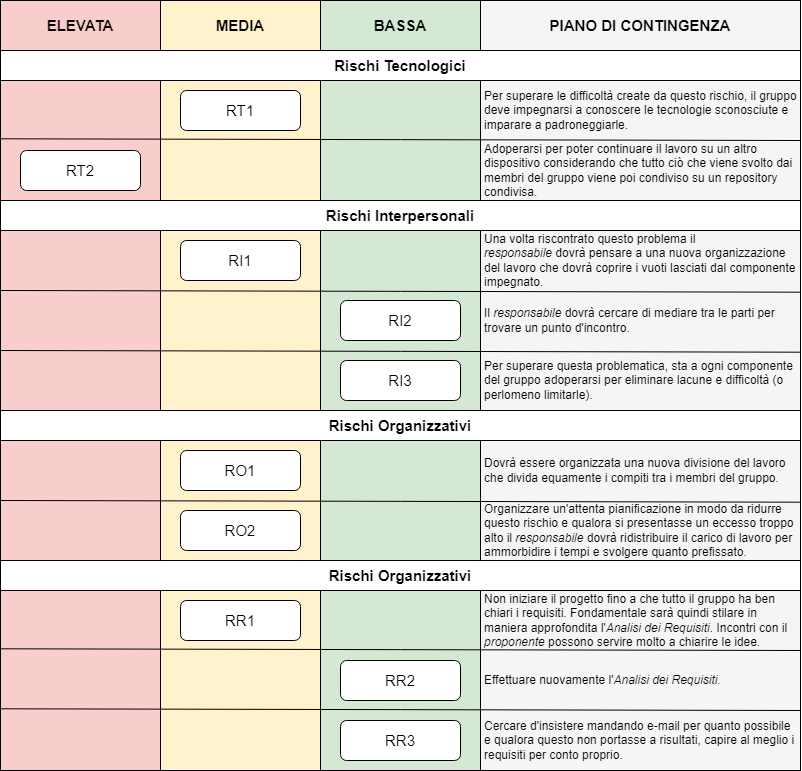
\includegraphics[scale=0.6]{immagini/piano_di_contingenza.png}
  \caption{Piano di contingenza}
\end{figure}